\documentclass[10pt, a4paper, twoside]{article}

% Set up the standard margins for the document
% 42.2 left & 15.5 right is same as Forsling, Neymark
% 21.3 top  & 20 bottom is same as Olofsson
\usepackage[left=25.5mm, right=25.5mm, top=21.3mm, bottom=20mm]{geometry}

% Input file character encoding (kinda useless if we don't
% use åäö and stuff, but it doesn't hurt to have it)
\usepackage[utf8]{inputenc}
%\usepackage[swedish]{babel}
\usepackage{caption}
\usepackage{subcaption}
% Block Comments
\usepackage{comment}

% No indentation in new paragraph
\usepackage{parskip}

% To include graphics
\usepackage{graphicx}

% More mathematical symbols and fonts
\usepackage{amsmath}
\usepackage{amsfonts}
\usepackage{amssymb}

% Simple list
\usepackage[ampersand]{easylist}
\ListProperties(Hide=100, Hang=true, Progressive=5ex, Style*=$\bullet$ ,
Style2*=-- ,Style3*=$\circ$ ,Style4*=\tiny$\blacksquare$ )


% Clickable internal links
\usepackage{hyperref}
\usepackage[all]{hypcap} % without this the link takes you to the caption, not the top of the image
\hypersetup{ % Settings for links in documnet
	setpagesize = false, % Don't allow hyperref to change page size. Tips från Micke Olofsson
	colorlinks = true,   % No boxes around links
	linkcolor = black,citecolor = black,filecolor = black,urlcolor = black, % don't color links
}

% To include to first page pdf file
\usepackage{pdfpages}

% Add section number to equation and figure number (ex: 5.11 instead of simply 11)
\numberwithin{equation}{subsection}
\numberwithin{figure}{section}
\numberwithin{table}{section}

% Show program code listings in document
\usepackage{listings}

%
% Header stuff
%
\usepackage{fancyhdr}
\setlength{\headheight}{15pt}

\fancyhf{}
\fancyhead[LE, RO]{\thepage}
\fancyhead[RE]{TSBB15 2013: Project Report}
\fancyhead[LO]{3D Reconstruction and Camera Pose Estimation}

\fancypagestyle{plain}{ %
\fancyhf{} % remove everything
\renewcommand{\headrulewidth}{0pt} % remove lines as well
\renewcommand{\footrulewidth}{0pt}}
%
% End header stuff
%


\begin{document}

% First page

\includepdf{Cover/cover.pdf}


% Project identity page
\newpage
\pagestyle{fancy}
\pagenumbering{roman}
\setcounter{page}{2} % sets the current page number to 2 

\begin{center}
    \vspace*{4\baselineskip}

	\textbf{\huge PROJECT IDENTITY} \\
	\vspace*{0.5\baselineskip}
	Computer Vision, VT 2013, group 2 \\
	Department of Electrical Engineering (ISY), Link\"{o}ping University
	
	\vspace*{2\baselineskip}
	\textbf{\LARGE Participants}


	{\footnotesize 
	\begin{tabular}{|p{2.7cm}|p{5cm}|p{2cm}|p{3.4cm}|}
		\hline
			\textbf{Name} & \textbf{Responsibilities} & \textbf{Phone} & \textbf{E-mail} \\
		\hline
		Gustav Häger & Background modelling &  & gusha124@student.liu.se \\
		\hline
		Alexander Sjöholm & Kalman prediction, \newline Evaluation of results &  & alesj050@student.liu.se \\
		\hline
		Martin Svensson & Foreground segmentation & 070--289\,01\,49 & marsv106@student.liu.se \\
		\hline
		Mattias Tiger & Object identification &  & matti166@student.liu.se \\
		\hline
	\end{tabular}
	}

{\footnotesize 
\textbf{E-mail list to the group}: marsv106@student.liu.se \\
\vspace{1\baselineskip}

%\textbf{Customer}: Some Guy, Link\"{o}ping University \\
%\textbf{Customer contact}: 333--33\,33\,33, 070--333\,33\,33, Fax: 013--33\,33\,33, some_guy@some_domain.se \\
\textbf{Project supervisor}: Fahad Khan, Link\"{o}ping University, fahad.khan@liu.se \\
\textbf{Course leader}: Per-Erik Forssén, 013--28\,56\,54, per-erik.forssen@liu.se \\
}

\end{center}



% table of contents
\newpage
\tableofcontents
\listoffigures
%\listoftables

% list of figures
%\newpage
%\listoffigures


% Document history page
\newpage
\vspace*{5\baselineskip}

\begin{center}
\textbf{\LARGE Document history}

{ \footnotesize 
\begin{tabular}{|p{1cm}|p{2.0cm}|p{5cm}|p{1.5cm}|p{2cm}|}
	\hline
	\textbf{Version} & \textbf{Date} & \textbf{Changes} & \textbf{Sign} & \textbf{Reviewed} \\
	
	\hline
	0.1 & 2013--04--29 & Initial draft & MS & \\
	\hline
	1.0 & 2013--05--16 & Final Report & Group 2 & \\
	
	\hline
	 &  &  &  &  \\
	
	\hline
\end{tabular}
}
\end{center}


% Blank page
%\newpage
%\thispagestyle{empty}
%\mbox{}



%
% Content start
%
\newpage
\pagenumbering{arabic}

\newpage
\section{Introduction}
This document is the final documentation of a mini-project performed as a part of the course Computer Vision (TSBB15) at Linköping university. The purpose of the project is to implement a tracker capable of handling occlusion, shadows and changes in the background. Object tracking is, in computer vision, defined as the process where moving objects are located in a image sequence. The project goal was to create a real-time tracker to work on e.g. a surveillance camera and track the people and objects in its view. The application was implemented in C++ using the OpenCV API.

The purpose of this document is to provide a thorough description of how the application was created and the problems encountered during the implementation work.


\section{System description}
\label{sec:system_description}
The system implementation is divided into four main modules, Feature extraction, Pose estimation, Non-linear optimization and 3D visualization.

\begin{figure}[htb]
	\centering
	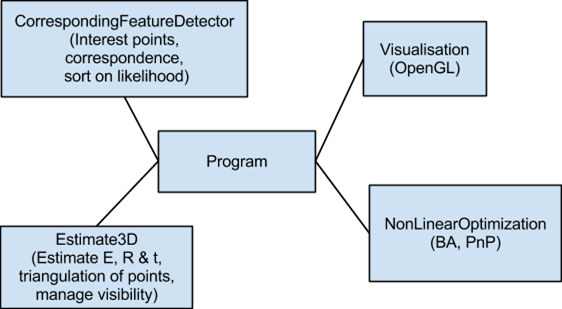
\includegraphics[width=110mm]{images/system_modules.png}
	\caption{\textit{Modules of the system}}
	\label{fig:block_overview2_fig}  %Skapar referens till figuren
\end{figure}

First feature extraction using Harris is performed as a preprocessing step on all images. These are used to calculate pairwise image point correspondences using SIFT.

Then an iterative process is performed cycling though all camera-pairs, each consisting of two parts. The first part contains an initial camera pose estimation, of the new camera, using the essential matrix estimated from F using the Gold standard algorithm. The camera pose is then improved using PnP on all previously known 3D-points and over all cameras. An initial 3D-point triangulation is then calculated.
The second part is a bundle adjustment over all current 3D points and cameras by the means of a non-linear optimization.

When all camera poses and estimated 3D-points have been iteratively added and optimized the result is rendered using OpenGL.

\begin{figure}[htb]
	\centering
	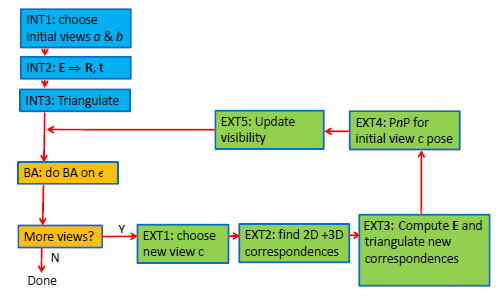
\includegraphics[width=120mm]{images/data_flow.png}
	\caption{\textit{Data flow between modules.}}
	\label{fig:block_overview_fig}  %Skapar referens till figuren
\end{figure}


\newpage
\subsection{Main Program}
\label{sec:main_program}
The main program is composed of two parts. The first one is initiation part, where the modules are declared, parameters specified, and movie clip loaded. The second one is the main loop, where the actual program is executed.


\subsubsection{Main loop}
When the program is started and the initiation is done the program is set to run until the end of the specified movie sequence. For each frame in the sequence, the Background model is updated and a probability map matrix containing information about what pixels are part of the background is created. After the probability map has been created, the foreground processing module is called upon to perform some noise removal and to detect all the interesting regions in the probability map (the regions that are likely to be part of the foreground). 

Once all the interesting regions are labeled, the identification module takes all the created objects in the current frame and associates them with the proper ID. This is done by comparison with the objects in the previous frame.

To help in the labeling process we use a Kalman predictor, that predicts the position of the each object in the next frame. The Prediction module is called upon after the identification is done.

Once all the processing in the module is finished the objects in the current frame are drawn in the current frame as bounding boxes with velocity vectors, position in pixel coordinates and ID numbers.


See code in appendix \ref*{sec:Main_code}. %referens till kod, ger klickbar l�nk.

\begin{figure}[htb]
	\centering
	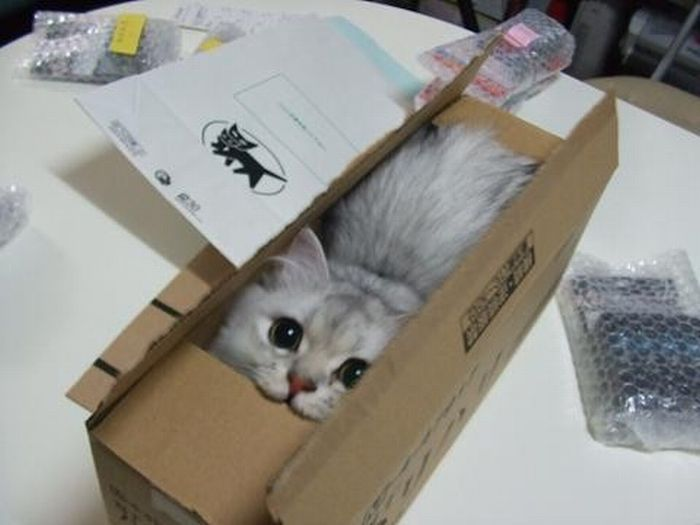
\includegraphics[width=\linewidth]{images/acatisfinetoo}
	\caption{\textit{Some flowchart of main program.}}
	\label{fig:MainProgram_fig} %Skapar referens till figuren
\end{figure}



\newpage
\subsection{Data structures}
\label{sec:data_structures}
In order to keep a good structure on the program and a logical separation of functionalities, several data structures have been created.

\begin{figure}[htb]
	\centering
	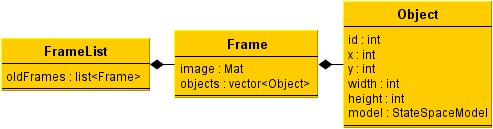
\includegraphics[width=150mm]{images/data_structures_uml.png}
	\caption{\textit{UML diagram of the main data structures. A video is represented by a FrameList, containing each Frame of the video. Each such Frame contains the detected objects in that image and each object contains spatial information, a unique id and a StateSpaceModel used for the Kalman filter prediction}}
	\label{fig:UML_fig} %Skapar referens till figuren
\end{figure}

%\subsubsection{ProbabilityMap}
%DErpa derpa derpa derpa. DErpa derpa derpa derpa.DErpa derpa derpa derpa.DErpa derpa derpa derpa.DErpa derpa derpa derpa.DErpa derpa derpa derpa.DErpa derpa derpa derpa.
%DErpa derpa derpa derpa.DErpa derpa derpa derpa.DErpa derpa derpa derpa.DErpa derpa derpa derpa.DErpa derpa derpa derpa.DErpa derpa derpa derpa.DErpa derpa derpa derpa.
%DErpa derpa derpa derpa. See code in appendix \ref{sec:ProbMap_code}. \cite{CVBook} % reference to bilbliography

\subsubsection{Object}
The \emph{Object} class represents a moving object in the scene. The information stored about the objects is ID, position, velocity, and bounding box. This information is what is processed in the object identification and prediction models. 

\subsubsection{Frame}
The \emph{Frame} class contains the current image as well as the probability map. Both if these are stored as \emph{cv::Mat}. The image is used for creation of the probability map as well as drawing the bounding boxes. From the probability map The foreground processing module finds and creates Objects that are stored in a vector. To draw the objects and their bounding boxes in the image, the function \emph{DrawObject} is called with the appropriate color. \ref{fig:UML_fig}. %Figurreferens

\subsubsection{FrameList}
The \emph{FrameList} class manages data sources (video) and provides frames sequentially as well as a history of previous frames. It contains methods for displaying the current frame and various interesting/useful information.






\newpage
\subsection{Correspondence Extractor}
\label{sec:point_extractor}
To get this machinery going it is necessary to find points in the images that are interesting to look at and follow through out the sequence. It is the correspondences between points in different images that will provide the information needed to reproduce the sequence in 3D. 

\subsubsection{Feature Extractor}
The feature extraction was carried out using Harris feature detector. This method uses the local structure tensor to sort out interesting parts of the image according to \eqref{eq:Harris}. This will generate a function where the value in each point is the level if interest in that local region. To select points one can threshold this at an appropriate level and morphologically shrink it to points. Besides the level of threshold one may also be interested in the closest distance between feature points. 

To be able to estimate the fundamental matrix of an image pair it is important to have known points all over the images. It is however not necessary to have more than seven corresponding points to calculate minimal estimate the fundamental matrix, also the calculation complexity will be reduced with fewer points. This motivates the finding few, properly spread out feature points. 

\begin{equation}
\label{eq:Harris}
C_{Harris} = det(A) - \kappa \cdot trace^2(A), \hspace{1cm} \kappa \approx 0.04
\end{equation} 

\begin{equation}
\label{eq:StructureTensor}
A =  \begin{bmatrix}
	   \langle \frac{\partial I}{\partial x} \rangle^2 &  \langle \frac{\partial I}{\partial x y} \rangle \\
	   \langle \frac{\partial I}{\partial x y} \rangle & \langle \frac{\partial I}{\partial y} \rangle^2
	  \end{bmatrix}
	  , \hspace{1cm} I = image
\end{equation}

\begin{figure}[htb]
	\centering
	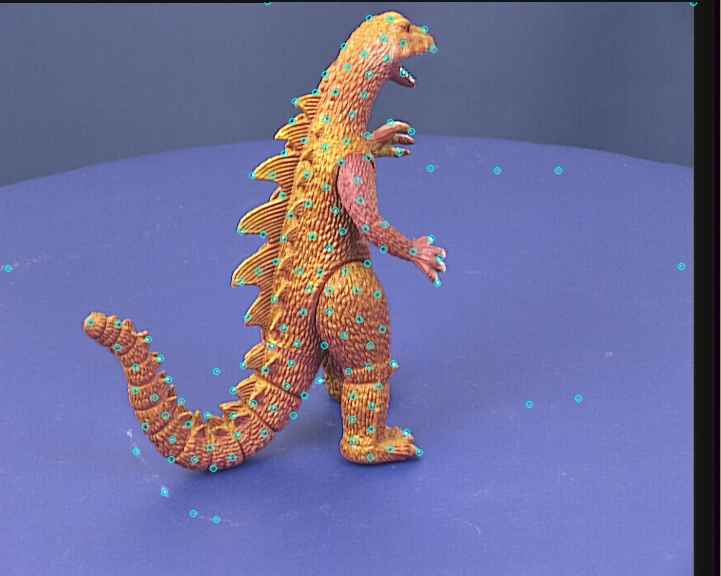
\includegraphics[width=110mm]{images/FeatureDetection.png}
	\caption{\textit{Feature points indicated with small circles. Notice the even distribution on the dinosaur body.}}
	\label{fig:FeaturePoints} %Skapar referens till figuren
\end{figure}

\subsubsection{Descriptor Extractor}
For all of the detected feature points a descriptor is calculated. This is done to be able to compare the features in different images. In this project the SIFT (Scale Invariant Feature Transform) descriptor is used. It is very effective in reducing unwanted effects of changes in illumination, scale and rotation. The way the descriptor work is that it calculates a series of histograms from gradient magnitude and orientation values from a small region around the feature point. The histograms are stored in a high dimensional vector, that once it has been normalized is the finished SIFT descriptor.

\subsubsection{Matching}
Finally, to find the correspondences between feature points in different images, the SIFT descriptors are compared between all feature points in the images. The descriptors that are most alike are chosen as a pair. There is also a check done to see that the found match is the closest possible match. This is done to remove potential outliers. A final check to get rid of matches that still slip through the first test is done in a euclidean distance thresholding. Points are not allowed to match on a to great distance.

Later in the pipeline a RANSAC (Random Sampling Consensus) algorithm is used to remove outliers while estimating the fundamental matrix, $F$, between images. The fundamental matrix defines a necessary but not sufficient constraint for corresponding feature points called the epipolar constraint, \ref{eq:EpipolarConstraint}. If a point pair diverge to far from zero it is discarded.

\begin{equation}
\label{eq:EpipolarConstraint}
y_1^T \boldsymbol{F} y_2 = 0
\end{equation} 

\begin{figure}[htb]
	\centering
	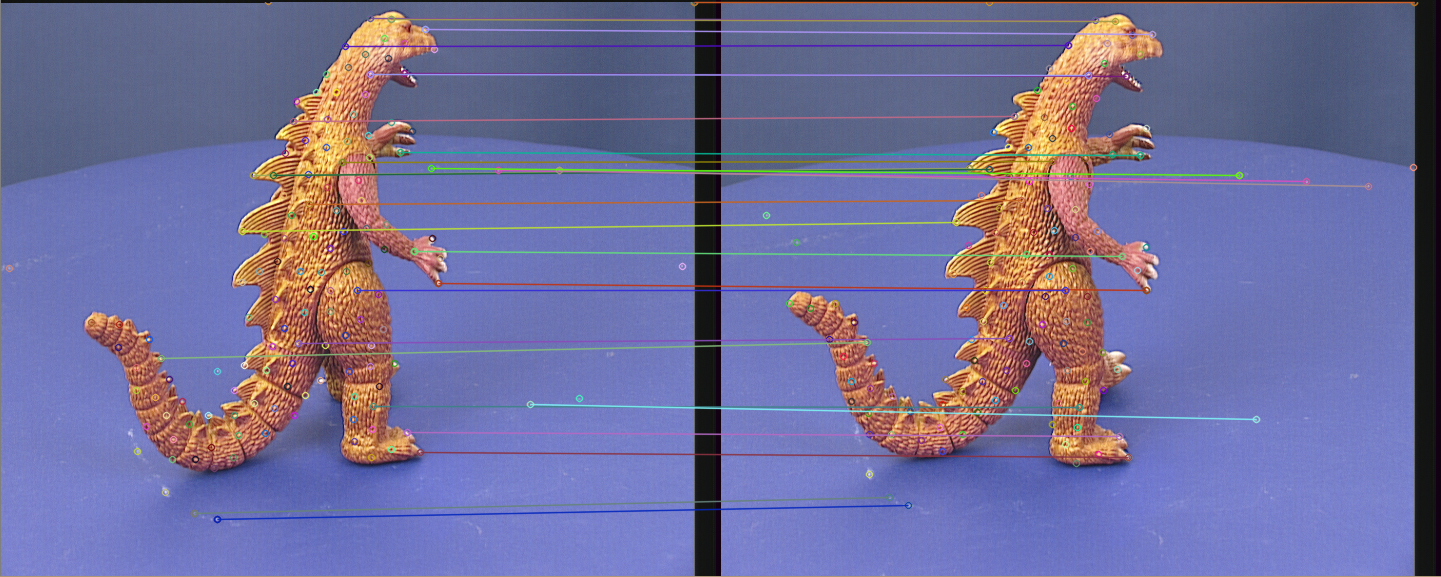
\includegraphics[width=\textwidth] {images/CorrespondenceDetection.png}
	\caption{\textit{Correspondences indicated with lines. Circles without a line attached lack correspondence.}}
	\label{fig:Correspondences} %Skapar referens till figuren
\end{figure}

\newpage
\subsection{Pose Estimation}
\label{sec:pose_estimator}
There are two cases of finding the pose of a camera. One is when there are only two cameras available, and the other one when there are several cameras already orientated to each other and one camera is being added to that group. In the first case an algorithm described in \cite{Klas} is being used. In the second a PnP (Perspective n-Point) algorithm is used.

\subsubsection{Alg. 5}
Given the fundamental matrix, $F$, for an image pair and the internal camera parameters, $K$, for the camera responsible for images, it is possible to estimate the two camera poses relative one another up to an unknown scale factor. This can be done in different ways, but since the camera is calibrated and the same for all images it is convenient to use algorithm 5 in \cite{Klas}. This uses a singular value decomposition of the essential matrix, \eqref{eq:EssentialMatrix} to find the translation, $t$, and rotation, $\boldsymbol{R}$, of camera two relative camera one. A minor drawback with the algorithm is that it produces four different combinations of rotations and translations that all need to be tested to find the correct one. For a more in detail description of the mathematical motivations of this algorithm see \cite{Klas}. 

\begin{equation}
\label{eq:EssentialMatrix}
\boldsymbol{E} = \boldsymbol{K}^T \boldsymbol{FK}
\end{equation}

\begin{equation}
\boldsymbol{U S V}^T = \boldsymbol{E}
\end{equation}

\begin{equation}
t_1 = v3, \hspace{1 cm}  \boldsymbol{V} = \begin{pmatrix}
										 |  & |  & |  \\
										 v1 & v2 & v3 \\
										 |  & |  & |
										\end{pmatrix}
\end{equation}

\begin{equation}
t_2 = -t_1
\end{equation}

This translation has an unknown scaling yielding the possibility of both plus and minus in sign. To find the rotation an auxiliary matrix, $\boldsymbol{W}$, is defined. Also to avoid mirroring in the rotation, the suggestions are multiplied with corresponding determinant.

\begin{equation}
\boldsymbol{W} = 	\begin{pmatrix}
					0  & 1 & 0 \\
					-1 & 0 & 0 \\
					0  & 0 & 1
					\end{pmatrix}
\end{equation}

\begin{equation}
\hat{\boldsymbol{R}}_1 = \boldsymbol{U W }^{-1} \boldsymbol{V}^T
\end{equation}

\begin{equation}
\hat{\boldsymbol{R}}_2 = \boldsymbol{U W }^{-T} \boldsymbol{V}^T
\end{equation}

\begin{equation}
\boldsymbol{R}_1 = det(\hat{\boldsymbol{R}}_1) \hat{\boldsymbol{R}}_1 
\hspace{2 cm}
\boldsymbol{R}_2 = det(\hat{\boldsymbol{R}}_2) \hat{\boldsymbol{R}}_2
\end{equation}

\begin{equation}
\boldsymbol{C}_{ij} = (\boldsymbol{R}_i | t_j)
\end{equation}

To find out which combination to chose, one corresponding point is chosen from the image pair. This point is then triangulated for the four camera pairs. Three of these triangulations should end up with the triangulated 3D behind the camera leaving only one camera left which is the one we choose. 

\subsubsection{PnP}
The PnP algorithm is used to fit an external camera to an existing set of cameras with corresponding triangulated 3D points. The algorithm tries to adjust the new camera's rotation and translation to minimize the re-projection error of the existing 3D points that by 2D correspondence are known to exist in the new camera as well. In the this procedure there is an optional outlier removal part where points producing too large re-projection errors are discarded from future 3D reconstruction. 

\newpage
\subsection{Non-linear Optimizer}
\label{sec:nonlin_optimizer}
There are three points in the reconstruction pipeline where nonlinear optimization is performed. In all three cases the optimization is performed using the levmar API \cite{levmar}. Levmar uses the Levenberg-Marquardt non-linear optimization algorithm to optimize a specified residual function, in this case re-projection errors of 3D points. The reprojection error is the distance, in pixels, between the projected 3D point and the corresponding point in the image plane. There are, in the implemented 3D-reconstruction pipeline, three instances where these highly non-linear functions are optimized over up to one thousand variables. With the Levmar API only accepting a residual function that take double arrays as both in and outputs, considerable preprocessing of the data is required.

\subsubsection{Rotation Parametrization}
In order to make it possible to find the optimal camera poses, the rotation matrices have to be parametrized. In this application they are parametrized using OpenCVs built-in Rodrigues' function, both in the PnP pose estimation and the bundle adjustment. This is a vector representation with the rotation angle described by the norm of the vector. The only ambiguity is the modulo $2\pi$ on the vector norm (ch.10.8 in \cite{Klas}), and by providing good initial guesses for the pose estimation, this is not an issue.

\subsubsection{Gold Standard estimation of F}
The function computing the gold standard refinement step is implemented as described in alg. 11.3, step (iii) in \cite{HZ}. The function takes, as an input, an initial guess of the F matrix, two projection matrices and vectors containing 2D and 3D correspondences. All input data is then preprocessed and re-arranged to fit the optimization API. The cost function described in equation \eqref{eq:GS} below is optimized over the twelve parameters of the projection matrix $P_2$ as well as the 3D-point coordinates, $p^{3D}$. 

\begin{equation}
\label{eq:GS}
\varepsilon^2 = \sum_{n=1}^{N} (p_{1,n}^{2D} - \textbf{P}_1p_{n}^{3D})^2 + (p_{2,n}^{2D} - \textbf{P}_2p_{n}^{3D})^2, \hspace{1cm} \textbf{P}_1 = [\bf{I} | \bf{0}]
\end{equation} 

For more in for on how the rest of the steps in the gold standard algorithm are implemented, see section \ref{sec:pose_estimator}.
\newpage

\subsubsection{Solving the PnP}
In the PnP the camera pose (rotation and translation) is estimated by minimizing the re-projection error of the visible 3D points.

In order for the data to fit the levmar interface and minimize the number of parameters the rotation matrices of each view is parametrized, as mentioned above, using the OpenCV Rodrigues' parametrization. Rotations and translations for each view are then stacked in a vector, along with all currently available 3D points. The second step is to make sure the residual function has access to all needed data, for example the visibility function and point correspondences.

The resulting cost function, to be minimized over \textbf{R} and \textbf{t} is

\begin{equation}
\label{eq:PnP}
\varepsilon^2 = \sum_{n=1}^{N} (p_n^{2D} - \textbf{KC}p_{n}^{3D})^2, \hspace{1cm} \textbf{C} = [\bf{R} | \bf{t}]
\end{equation} 

\subsubsection{Bundle Adjustment}
Th largest and most time-consuming use of the non-linear optimizing module is in the bundle adjustment step of the 3D-reconstruction pipeline. The bundle adjustment function refines the estimates of both camera poses (rotation + translation) and location of 3D points for all views. 

The residual function simply, for each view, calculates the re-projection error of all 3D points visible in that view, i.e the pixel distance of the reprojected 3D points to the actual image points used in the triangulation. In the equation below, $V$ denotes the number of views, $N_v$ the number of points visible in each view, and $p_{v,n}$ the corresponding image points. This expression is then minimized over all $p^{3D}$ as well as all rotations and translations. 

\begin{equation}
\label{eq:BA}
\varepsilon^2 = \sum_{v=1}^{V}\sum_{n=1}^{N_v} (p_{v,n}^{2D} - \textbf{KC}_vp_{v,n}^{3D})^2, \hspace{1cm} \textbf{C}_v = [\textbf{R}_v | \textbf{t}_v]
\end{equation} 


The number of outputs from the residual function scales rapidly with the number of views, as each view gives an additional $ 6 + 2N_v $ observations, where $ N_v $ is the number of 2D inliers in view $v$.


\newpage
\subsection{3D Visualization}
\label{sec:3d_visualization}
This module visualizes the calculated points and the camera positions relative to the position of the first camera. This part of the program is written on top of the OpenGL graphics API.

It can be run as a stand alone program, or as a last step in the 3D-reconstruction pipline. In the standalone case it will read the output files generated by the reconstruction pipeline. Using the keyboard a user can then step between the added cameras, with or without the bundle adjustment step done.

It is also possible to alter the scale of the points and cameras, as there is no automatic scaling in place and the points are drawn as colored spheres.

%massa bilder här, nån får ta och "fota" dem.

\subsubsection{Visualization}
The estimated 3D-points are plotted as textured/colored spheres, using the color from the image where the corresponding interest point was first detected, or a region surrounding the point. (this looks rather bad however)

Cameras are plotted as cones pointing toward the point cloud.

\begin{figure}[htb]
	\centering
	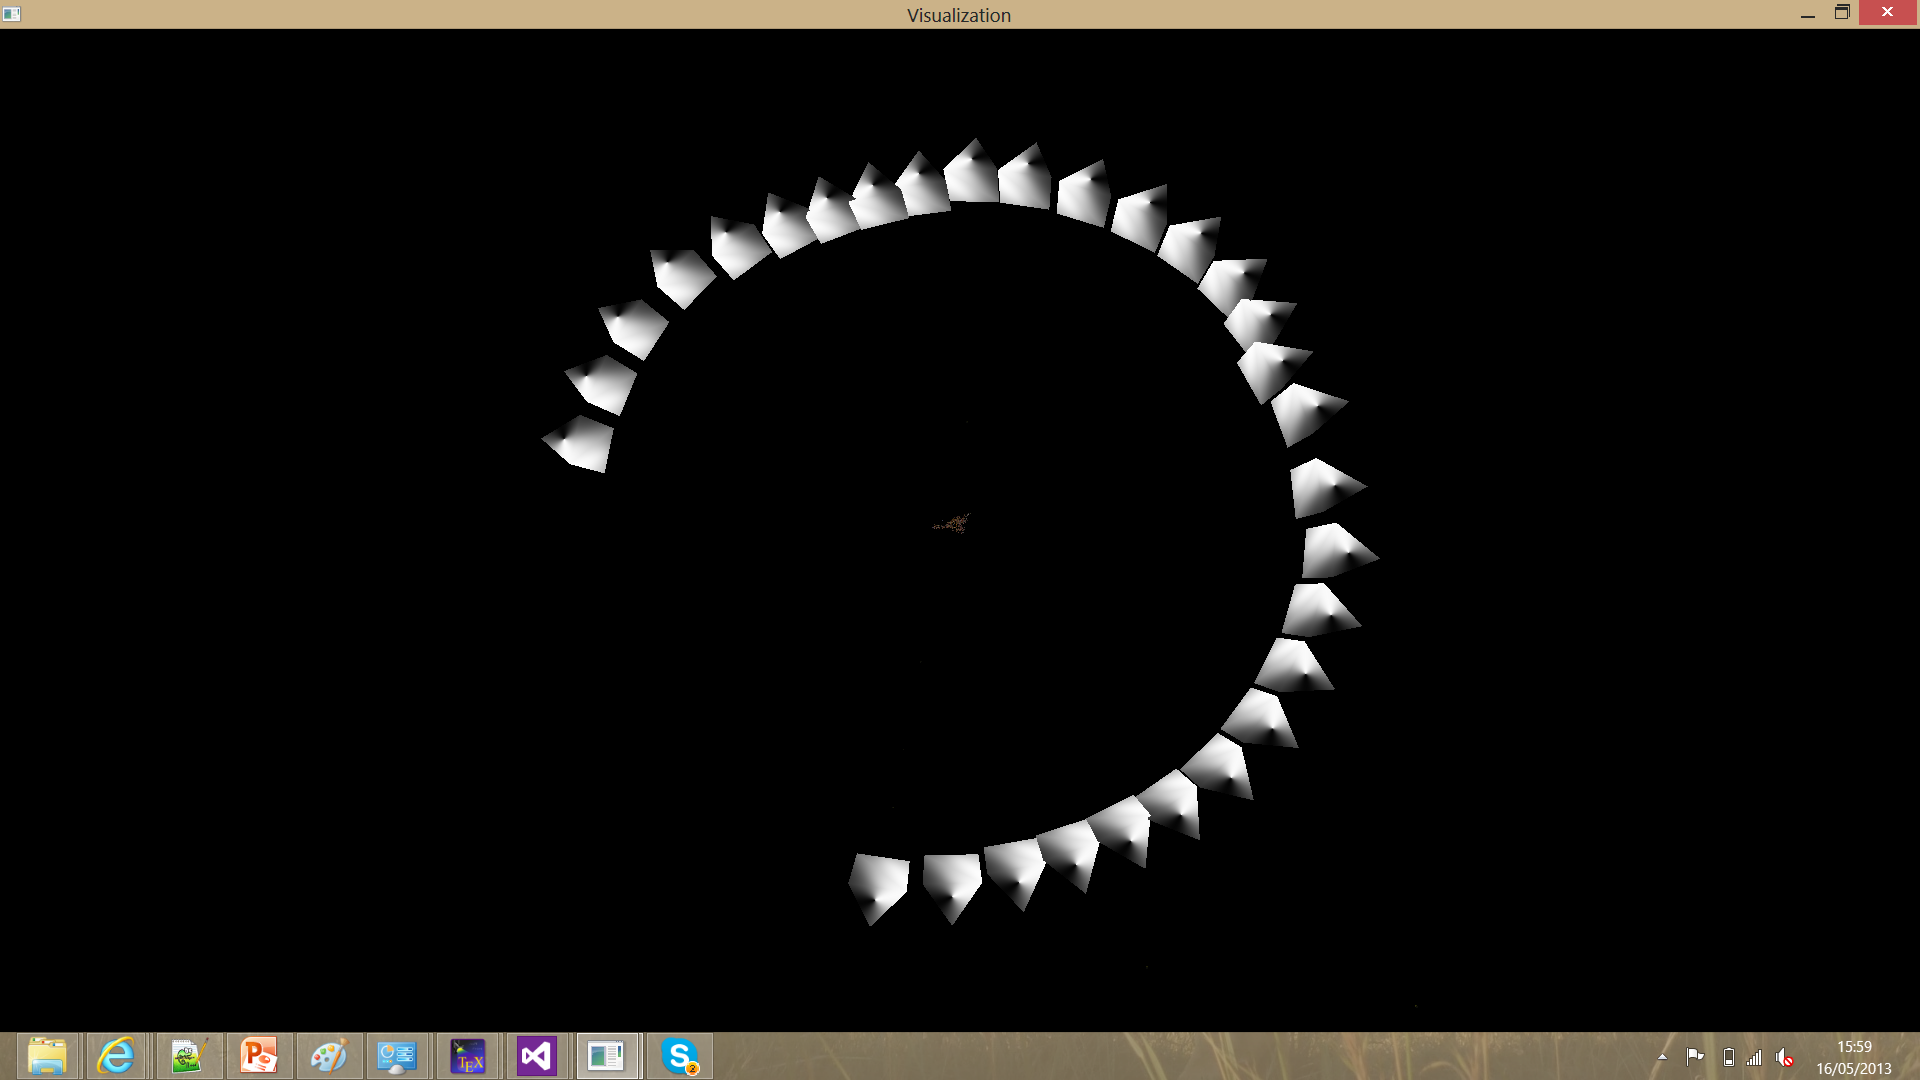
\includegraphics[width=110mm]{images/camRingLots.png}
	\caption{\textit{some cameras}}
	\label{fig:camRingLots}  %Skapar referens till figuren
\end{figure}

\begin{figure}[htb]
	\centering
	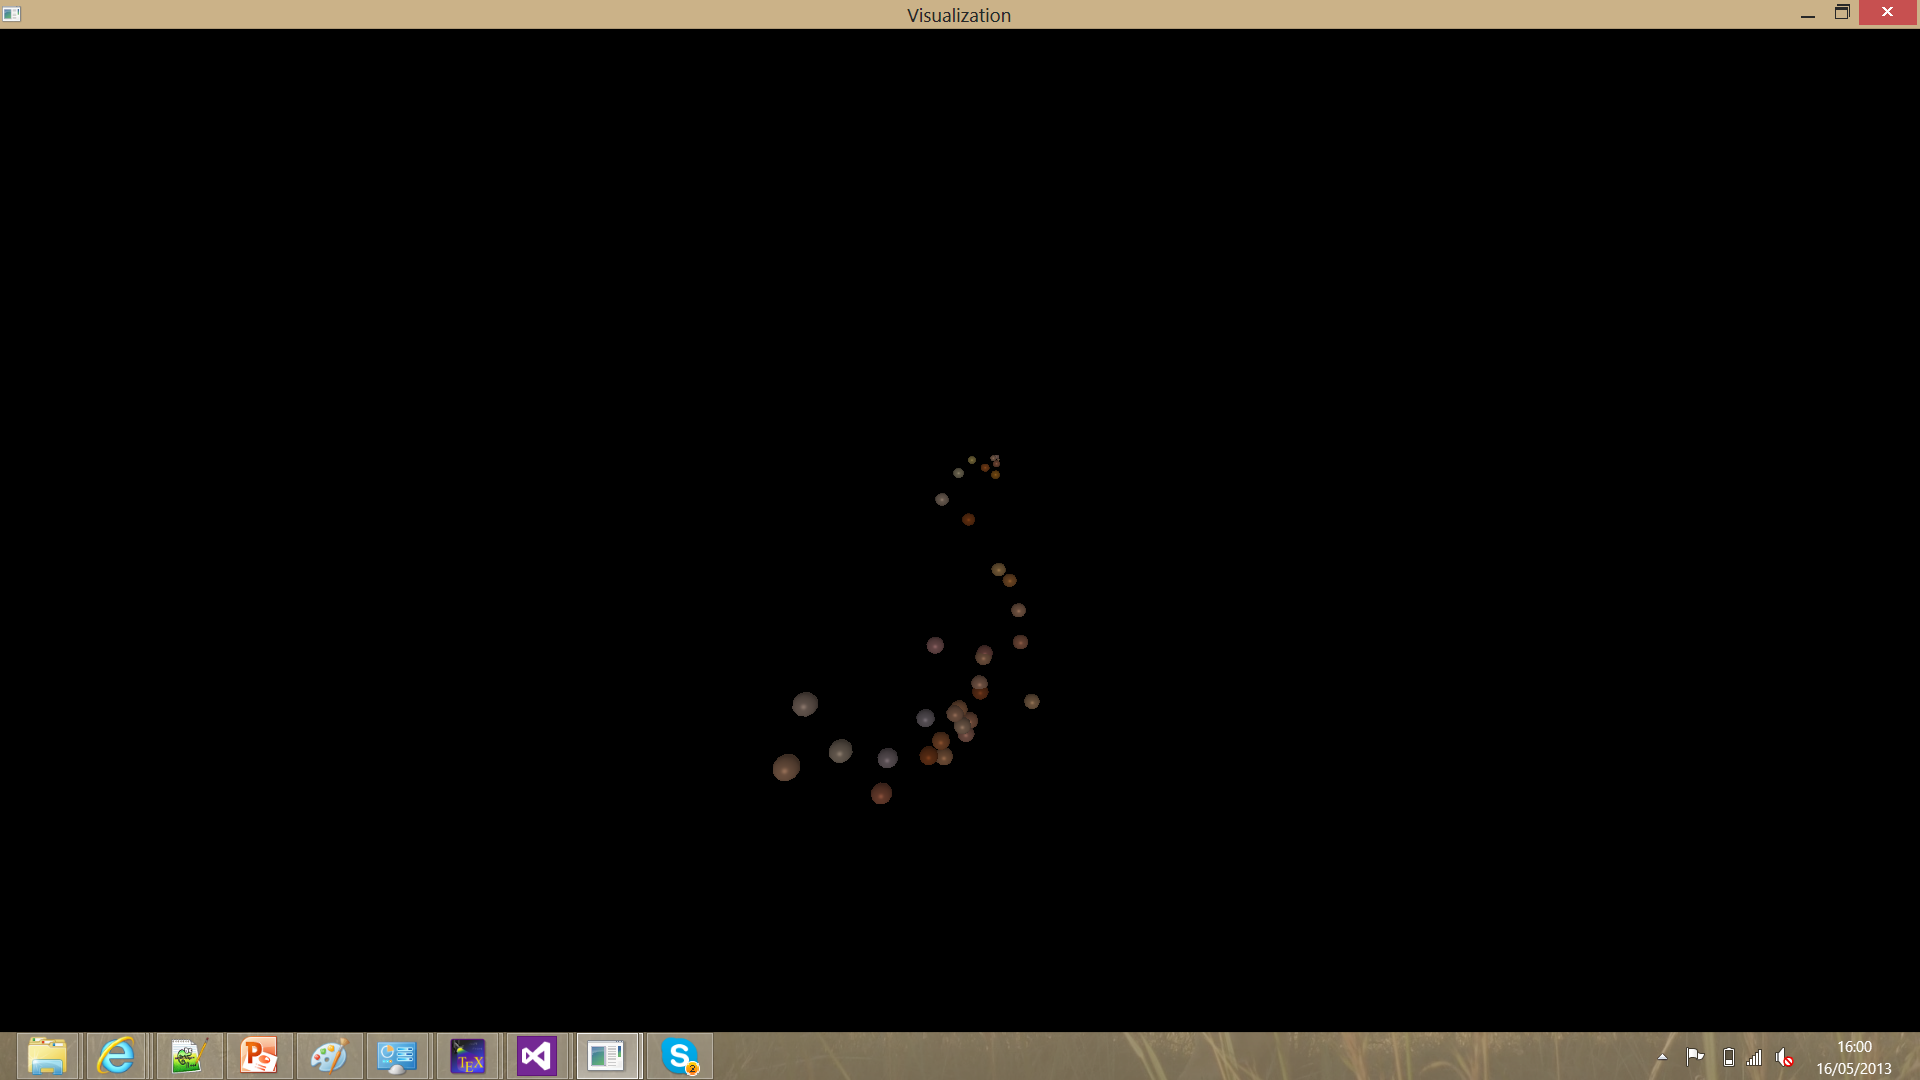
\includegraphics[width=110mm]{images/pointCloudFewCam.png}
	\caption{\textit{The dinosoaur with only a few cameras, very poor depth accuracy}}
	\label{fig:camRingLots}  %Skapar referens till figuren
\end{figure}

The main purpouse of the visualization modue is to compare 


\subsubsection{File managing}
Each iteration of the reconstruction pipeline produces two files, one with the reconstruction state before the bunle adjustment and one after. The files contain all detected 2D correspondances, the calculated fundamental matrix, and the known 3D points. The data is saved as text, to make inspection easier.


\newpage
\section{Results}
\label{sec:results}
In this section the results of the project is summarized for some sequences chosen together with the other group. The sequences, as well as the ground truth used are provided by the EC Funded CAVIAR project, \cite{CAVIAR}.

\subsection{Evaluation Scores}

\begin{table}
\centering
	\begin{tabular}{r | c | c | c }
		\emph{Sequence Name}		& \emph{MOTA} & \emph{MOTP} \\
		\hline \hline
		OneLeaveShop1front			& 0.56 & 5.01 \\
		OneLeaveShop2front			& 0.70 & 5.30 \\
		OneLeaveShopReenter2front	& 0.65 & 5.09 \\
		OneStopNoEnter2front 		& 0.85 & 5.48 \\
		WalkByShop1front 			& -0.66 & 7.96 \\
	\end{tabular}
	\caption{\textit{Tracking performance according to the MOTA and MOTP evaluation standards, as described in section \ref{sec:evaluation}.}}
	\label{tab:evaluation_performance}
\end{table}

\subsection{Parameters}

\begin{table}
\centering
	\begin{tabular}{r | c || c | c || c | c | c | c | c }
	&	\multicolumn{1}{|c||}{BG model} & \multicolumn{2}{c||}{FG Segmentation} & \multicolumn{4}{c|}{Shadow Detection} \\
		\hline
		\emph{Sequence Name} & \emph{Learning Rate} & \emph{Iterations} & \emph{Min Thickness} &\emph{$\tau_H$} & \emph{$\tau_S$} & \emph{$\alpha$} & \emph{$\beta$}\\ 
		\hline \hline
		OneLeaveShop1front			& 0.05 		& 3 & 3.5 	& 0.5 & 1 & 0.8 & 0.99\\
		OneLeaveShop2front			& 0.05 		& 3 & 4 	& 0.5 & 1 & 0.8 & 0.99\\
		OneLeaveShopReenter2front	& 0.05		& 4 & 4 	& 0.5 & 1 & 0.8 & 0.99\\
		OneStopNoEnter2front 		& 0.033		& 3 & 4 	& 0.5 & 1 & 0.8 & 0.99\\
		WalkByShop1front 			& 0.033 	& 4 & 8 	& 0.5 & 1 & 0.8 & 0.99\\
	\end{tabular}
	\caption{\textit{Parameters used to receive the evaluation results presented in table \ref{tab:evaluation_performance}.}}
	\label{tab:evaluation_parameters}
\end{table}


\subsection{Performance}


\subsection{Technical Conclusion}
The evaluation needs access to some sort of ground truth which is defined as the best possible achievable tracking output. Through out this part of the document an object is defined as a position by the ground truth and a hypothesis as the output from the tracker. The method only allows one-to-one correspondence between objects and hypothesis and in case of conflict the combination yielding the lowest total distance error is chosen.

\subsection{Conclusion}
MOTA is measure of accuracy with respect to how many mistakes are made by the tracker. It consists of four variables: misses, false positive, mismatches and number of objects. A miss is when no hypothesis is suggested close enough to an object. Close enough is defined by a threshold, T. This is the only design parameter in this method. If the distance between an object and the closest hypothesis is larger than T, the object yields a miss. If a hypothesis has no object within the threshold it results in a false positive error. One important feature of a tracker is the ability to keep objects identities correct. If this is not the case and an object is changing identity between frames one mismatch error is added for every change. The number of objects variable is defined as the total number of objects trackable according to the ground truth in the current frame. For a sequence the equation for MOTA is found in \eqref{eq:MOTA}.






\newpage
\section{Conclusions}
\label{sec:conclusions}
In general this project needed much better routines for testing and verification of indvidiual modules than the previous project, mainly due to far longer computational times involved.

\subsection{Correspondence Extractor}
It is important to do the correspondence extraction well, as this data is the basis for all further calculations. There are a couple of parameters that need to be tuned properly for every sequence. The features need be evenly distributed in the image the get enough information. It is for instance not good to have all features in a plane or many feature close to each other. This is solved with a minimum distance allowed between features. It is also important to look for features of the right size. This depends on resolution and image structure. To keep the number of features low and the quality high helps the program run faster. 

\subsubsection{Possible improvements}
Automatic parameter detection based on image analysis in some way would make the program more user friendly. At the moment it requires an experienced user. 

\subsection{Pose Estimator}
The pose estimator is very sensitive to the quality of the correspondences. It does not handle outliers or points on a plane very well. This corrupts the estimation completely since it cannot provide even rough estimates to the bundle adjustment optimization. However, as long as the outliers are removed and the points are spread out in more than two dimensions it works very well. 

Deducting which 3D-points were seen in the previous image it was possible to run PnP on the known 3D-points in order to improve the pose of the new camera significantly. Using this result it was possible to remove most problematic outliers by triangulating the new points and to threshold them according to their re-projection error. This both improved the result and increased the speed of the computations in the BA step as it was given a better initial estimate.

\subsubsection{Possible improvements}
If something about the camera trajectory is known one could possibly constrain the pose estimation and make it more robust.
Another possible improvement would be to find chains of corresponding points though out the image sequence which then should correspond to the same 3D-point. 
\newpage

Using as long chains as possible while still always have at least a minimum of image points in each image they could be cross-validated for each image and the worst points removed from the chains, splitting these, and resulting in possibly very high-quality estimates of trajectories of 3D-points captured in the image sequence. These chains could then be used in the pipeline resulting in a very sparse 3D-model with possibly very high camera pose estimation accuracy. The next step would then be to triangulate most other image points using these "known" cameras and building up a dense 3D-model. Additional verifications, validations and re-estimations of the camera-poses might be done in order to ensure that the estimated cameras poses are indeed very accurate. The speed up from this process could be very large, as well as the quality of the model perhaps!

\subsection{Non-linear Optimizer}
The non-linear optimization implementation performs well and no significant problems related to neither the pose representation, nor the representation of points or the visibility function were struck. The hardest part was to figure out how to convert all the data to fit the API, but once that was figured out, the implementation was very straight-forward, and the bundle adjustment part was not much harder to implement than the Gold Standard or PnP parts.

\subsubsection{Possible improvements}
The improvement that would yield the largest performance increase in the bundle adjustment would be making use of the lack of independence between views and drastically lower the computational load. The original thought was to use the sparseLM API \cite{sparseLM}. Unfortunately, due to lack of time, this was never implemented as it would require the representation of the visibility function to be remade completely. 

A second significant improvement would be to make use of the LAPACK API, that was highly recommended for use in combination with levmar, and said to speed things up significantly. It was, however, rather complicated and time consuming to set up, and these are the reasons it is not used in this implementation.

\subsection{3D Visualization}
Implementing this part of the system in OpenGL was perhaps not the wisest decision, as the amount of work and difficulty to debug OpenGL calls made progress rather slow.

It did however make it easy to implement project-specific functions into the visualizer without having to learn yet another API.

\subsubsection{Possible improvements}
It should be possible to color the points according to the image data they are extracted from. If more points where obtained it should be possible to draw them only as colored dots in space.

Further one might create a mesh between the detected points, to generate a full 3D-Model. It should then also be possible to texture it using data from the images to create a complete 3D representation of the original physical object.

Another improvement would be to add runtime settings to many of the options that are currently set in the source code, as recompiling the program every time the scale of the objects need to change is somewhat clumsy.
\newpage
%
% Bibliography
%

% Force a blank page so the bibliography starts on a new page.
% Comment out if not necessary
%\newpage
\thispagestyle{fancy}
\mbox{}
\newpage
\begin{thebibliography}{9}
\addcontentsline{toc}{section}{References} % Add an entry for this in the table of contents

\bibitem{CVBook}
	Sonka, M., Hlavac, V. \& Boyle, R. \\
	\emph{Image Processing, Analysis, and Machine Vision}.\\
	Toronto: Thompson Learning,\\
	cop. 2008, 3rd ed.,\\
	ISBN 0495244384.

\bibitem{levmar}
    Lourakis, M.I.A.\\
   \emph{levmar: Levenberg-Marquardt nonlinear least squares algorithms in {C}/{C}++}\\
     \verb+http://www.ics.forth.gr/~lourakis/levmar/+,\\
    Jul. 2004\\
    Accessed on May 14th 2005.
    
\bibitem{sparseLM}
    Manolis I.A. Lourakis\\
   ``Sparse Non-linear Least Squares Optimization for Geometric Vision,''\\
    \emph{European Conference on Computer Vision},\\
    vol.~2, 2010,
    pages~43-56 \\
    DOI \verb+http://dx.doi.org/10.1007/978-3-642-15552-9_4+

\bibitem{HZ}
	Hartley, R \& Zisserman, A\\
	\emph{Multiple View Geometry in Computer Vision}.\\
	Cambridge University Press, West Nyack, NY, USA \\
	March 2003, 2nd ed.\\
	ISBN 978--05--11--18711--7
	
\bibitem{Klas}
	Nordberg, K\\
	\emph{Introduction to Homogeneous Represenations and Estimation in Geometry}\\
	Apr. 2013\\
	Computer Vision Laboratory,	Department of Electrical Engineering\\
	Linköping University


	

%\bibitem{somePaper}
%	Q. Lastname,
%	``Some article title,''
%	\emph{Some scientific journal},
%	vol.~1337, no.~1337,
%	pp.~666--1337,
%	month.~1337.

\end{thebibliography}



%\lstinputlisting{code_files/Sigma_Delta_PSD_SNR_and_ENOB_calculations_INNAN_PILL.m}
%\end{comment}

\end{document}
